\documentclass[12pt]{article}
\usepackage{amsmath}
\usepackage{graphicx}

\begin{document}
\section*{Micro Controller State Machine}
The following state machine describes the various states
of the Ti Simple Link CC 3220 Micro controller.
\begin{figure}
\center
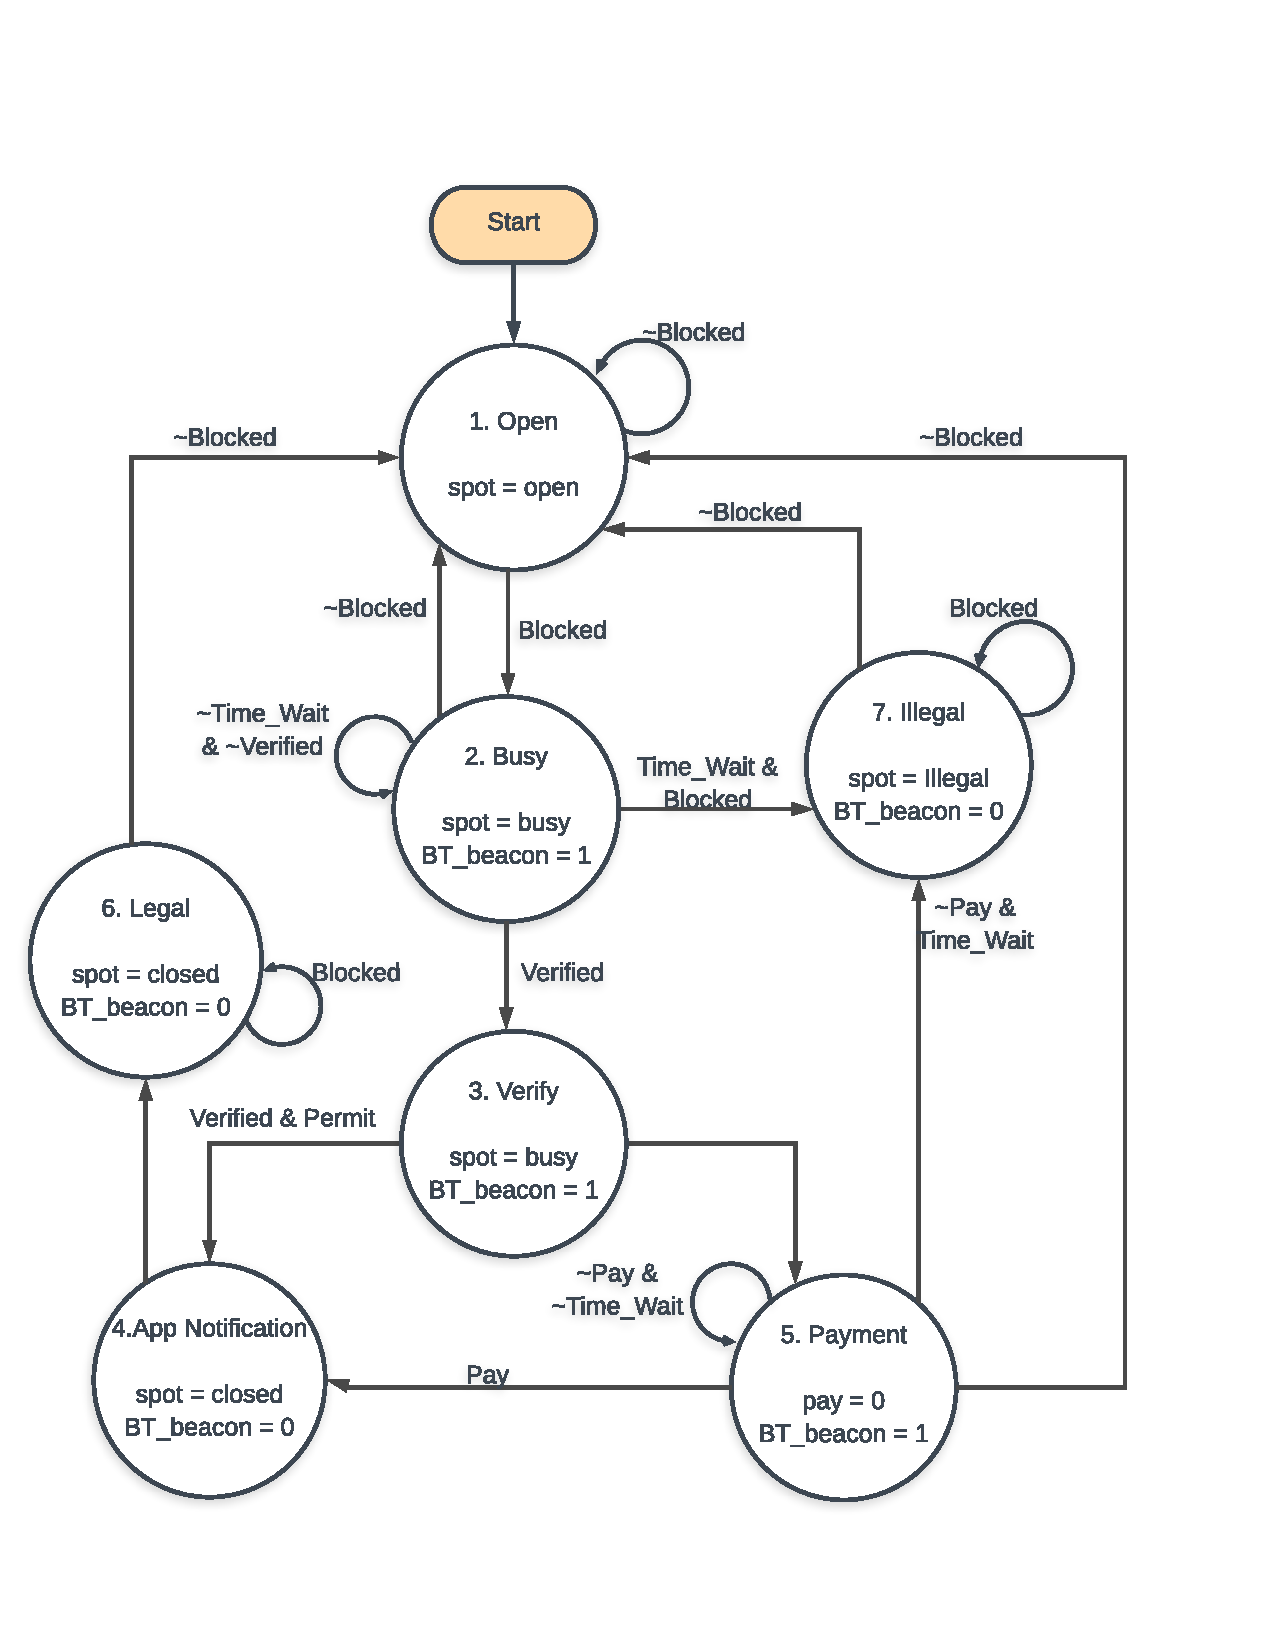
\includegraphics[scale=0.8]{SM.pdf}
\caption{Signal approximations for $F_s$ = 70}
\end{figure}

\begin{enumerate}
\item \textbf{Open} - This state is where the parking
spot is empty. The micro controller periodically checks 
for the sensor being blocked.

\item \textbf{Busy} - When the sensor is blocked, We wait for a little bit by a time of \verb|Time_Wait|. If the
sensor is no longer blocked, we had a fake detection, and
current state returns to state 1. Blue Tooth is turned on 
in this state so the app of a user's phone can read a blue tooth string and verify with the cloud. If the cloud successfuly verifys a user, it will signal the micro controller to enter the verified state. If the user does not have the app open or does not have a permit/account, or if the \verb|Time_Wait| expires, the state will change to the illegal state (state 7).

\item \textbf{Verify} - In this state the Cloud has signaled the micro controller that the user has been in the database. The cloud will then tell the micro controller and app if we need to get user payment or if no payment is needed if a user has a pre-paid permit. If the user has a permit, we go to state 4. If the user needs to make a payment, we go to state 5.
\item \textbf{App Notification} - A notification will be displayed on the app, 
and the spot will be marked as closed in the database. The
could will put a log to the transaction history will be placed in the database at this point. Lastly the state moves to the legal state.

\item \textbf{Payment} - When the user needs to make a payment, he/she will be shown their account balance and will authorize a payment. The funds will be deducted from the account balance and the state will change to state 4. If no payment is made, after a certain \verb|Time_Wait|, we will go to the illegal state (state 7). If the user decides to leave the space, we return to state 1.

\item \textbf{Legal} - When the user has been successfully validated, the micro controller stays in this state until the user leaves. The micro controller periodically checks to see if the spot is still blocked. When the spot is no longer blocked, we notify the Cloud and return to state 1.

\item \textbf{Illegal} - In this state, the user has either not made a payment or not verified a permit. A red led will turn on. The micro controller will stay in this state until the sensor is no longer being blocked.
\end{enumerate}

\end{document}